\chapter{Роздільна здатність}\label{cha:resolution}
\textbf{Роздільна здатність} - це вимірювання щільності дискретизації, роздільна здатність растрових зображень дає зв'язок між розмірами пікселів та фізичними розмірами.
Найбільш часто використовується вимірювання - ppi(pixel per inch), пікселів на дюйм.

Різниця між \textbf{ppi} та \textbf{dpi} - це різниця між пікселями та точками - пікселі можуть представляти кілька значень, тоді як крапка - це монохромне пляма чорнила або тонера одного барвника, виготовленого принтером.
Принтери використовують процес, який називається \textbf{напівтонування}, для створення монохромного малюнка, що імітує діапазон рівнів інтенсивності.

\section{Мега піксель}\label{sec:megapixels}
Мегапікселі відносяться до загальної кількості пікселів у захопленому зображенні, простішою метрикою є \textbf{растрові розміри}, які представляють кількість горизонтальних та вертикальних зразків у сітці вибірки.
Зображення зі співвідношенням сторін 4:3 із розміром 2048x1536 пікселів містить загалом 2048x1535 = 3145728 пікселів;
приблизно 3 мільйони, таким чином, це 3-мегапіксельне зображення~\cite{gimp:1}.

\begin{figure}
    \label{fig:image5}
    \centering
    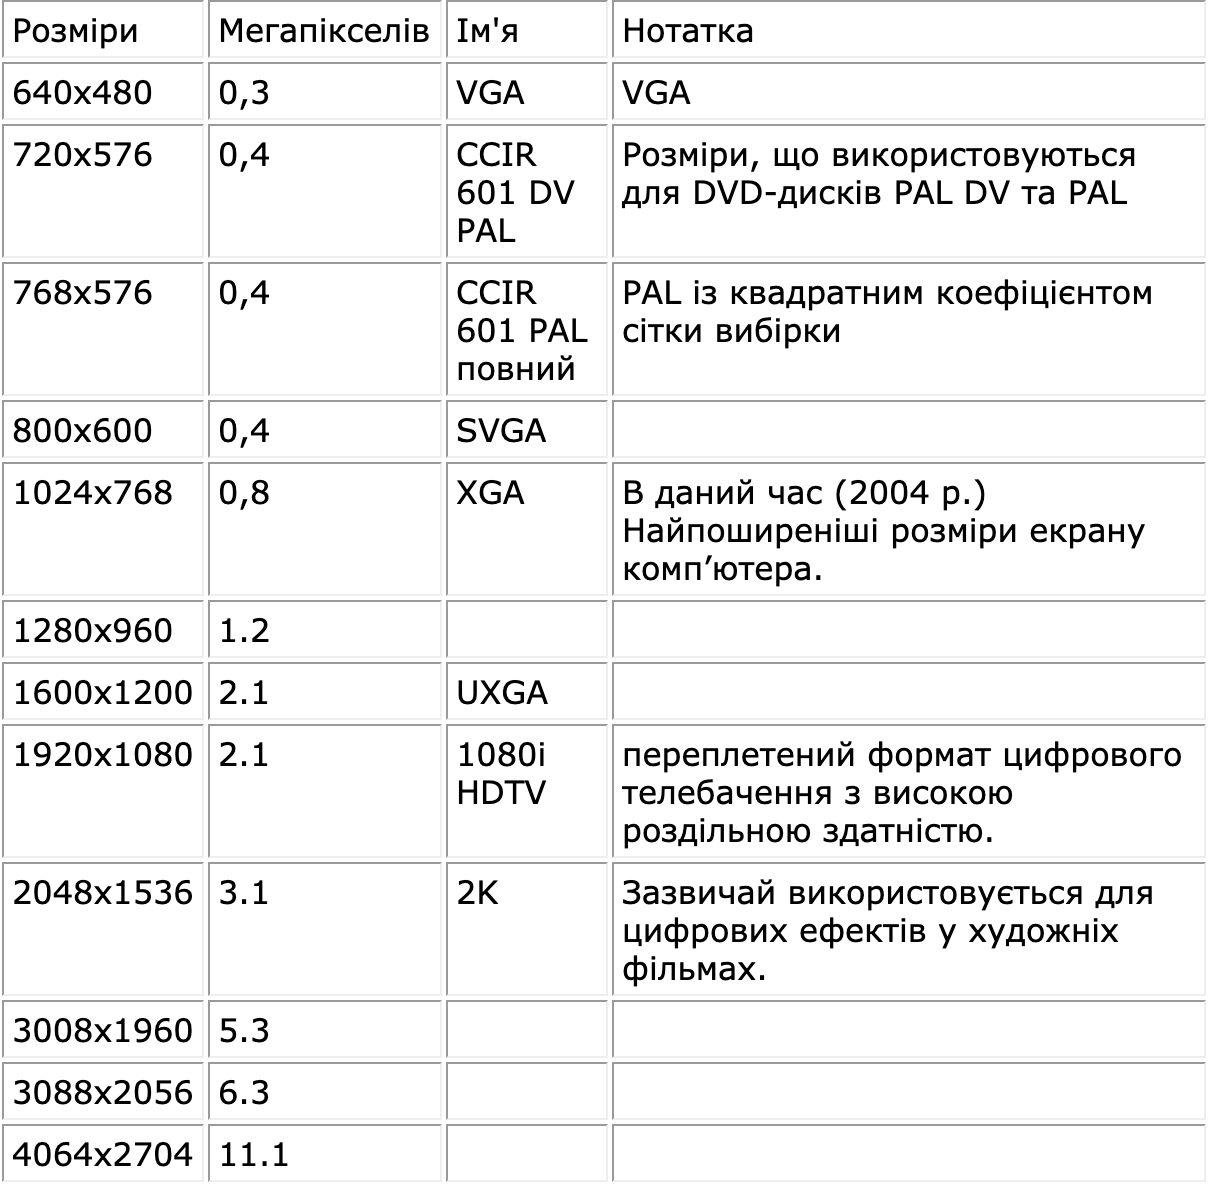
\includegraphics[scale=0.5]{image5.png}

    Рис. 5. Загальні растрові розміри
\end{figure}

\section{Масштабування / Передискретизація (Scaling / Resampling)}\label{sec:scaling_resampling}
Коли нам потрібно створити зображення з різними розмірами, ніж ми маємо, ми масштабуємо зображення.
Інша назва масштабування - передискретизація, коли алгоритми передискретизації намагаються відновити вихідне безперервне зображення та створити нову сітку зразків~\cite{gimp:1}.

\section{Зменшення масштабу зображення}\label{sec:downscaling}
Процес зменшення растрових розмірів називається децимацією (decimation), це може бути зроблено шляхом усереднення значень вихідних пікселів, що вносять вклад в кожен вихідний піксель~\cite{gimp:1}.

\section{Масштабування зображення вгору}\label{sec:upscaling}
Коли ми збільшуємо розмір зображення, ми фактично хочемо створити точки вибірки між вихідними точками вибірки у вихідному растрі, це робиться шляхом інтерполяції значень у сітці вибірки, ефективно вгадуючи значення невідомих пікселів.
При використанні цифрового масштабування камери камера використовує \textbf{інтерполяцію}, щоб вгадати значення, яких немає на зображенні.
